\documentclass[a4paper]{article}

\usepackage{cite}%多个文献引用
\usepackage{graphicx}
\usepackage{array}%调节表格行高
\usepackage{multirow,makecell}%多行表格
\usepackage{tabularx}%表格固定列宽
\usepackage{subfigure}
\usepackage{titlesec}%标题格式设置
\usepackage{amsmath}
\usepackage{amssymb}
\usepackage{tabularx}
\usepackage{makecell}
\usepackage{geometry}
\usepackage{float}
\usepackage{setspace}%行距包
\usepackage{siunitx}
\usepackage{mdwlist}
\usepackage{tabu}
\usepackage{enumerate}

\geometry{top=1.54cm,bottom=2.54cm,left=2.5cm,right=2.5cm}


\begin{document}
\begin{center}
\bf\Large
EE 105 Feedback Control Systems\par
Department of Electrical and Computer Engineering\par
Tufts University Fall 2018\par
Homework \#8\par   
\end{center}
\begin{table}[H]
\begin{center}
\begin{tabular*}{\textwidth}{@{\extracolsep{\fill}}lcr}
Name: {\it Shang Wang} &Student ID: {\it 1277417} &E-mail: {\it shang.wang@tufts.edu}\\
\hline
\end{tabular*}
\end{center}
\end{table}

\section{Problem 1}
First, lower a gain by the factor
$$
K = 0.5
$$
We have bode plot:
\begin{figure}[H]
\centering
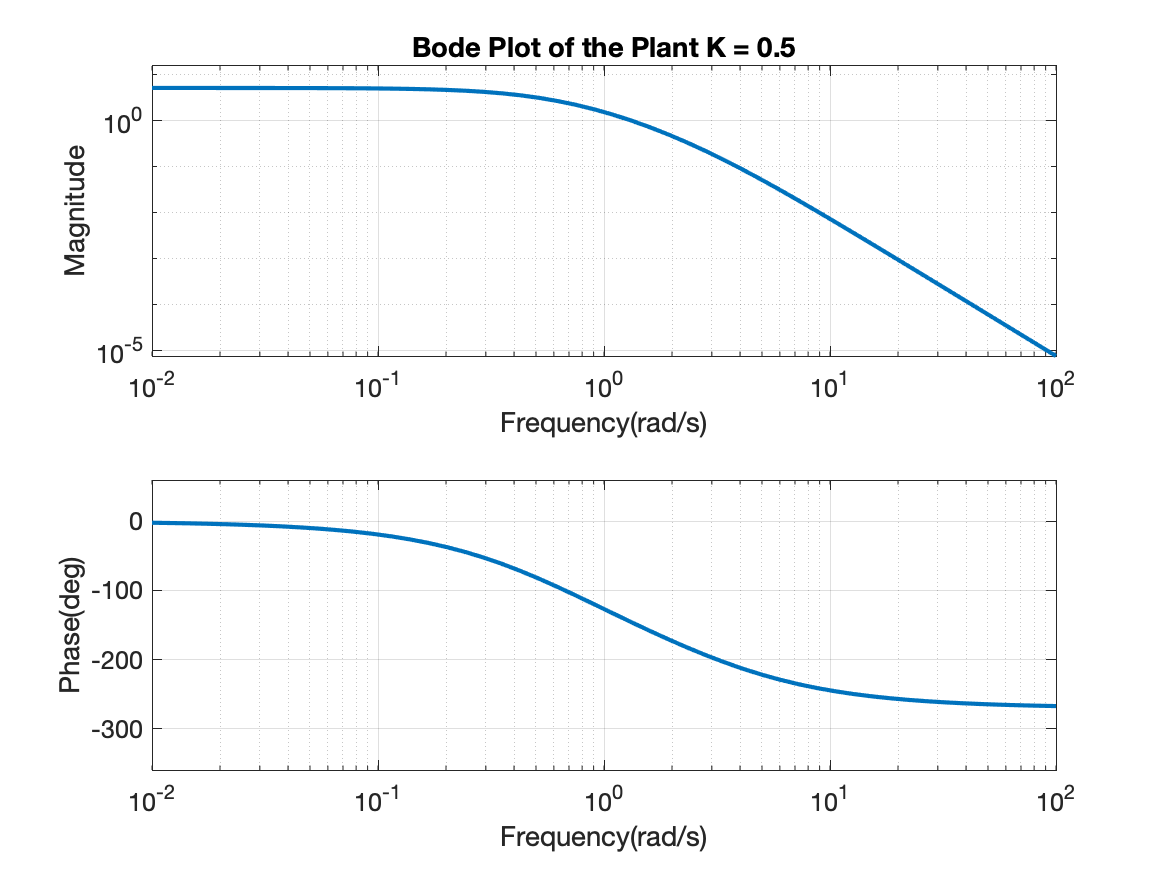
\includegraphics[width = 0.6\textwidth]{pic/0.png}
\end{figure}
\noindent Then use lag compensator to boost the DC gain in order to satisfy the steady state error. 
$$
D_{Lag} = \beta\frac{T_Is+1}{\beta T_Is +1}
$$
Where $\beta = 20$, $T_I = 5$, zero at $\omega_{lagz} = 0.2$, pole at $\omega_{lagp} = 0.01$
The bode plot of Lag Compensator
\begin{figure}[H]
\centering
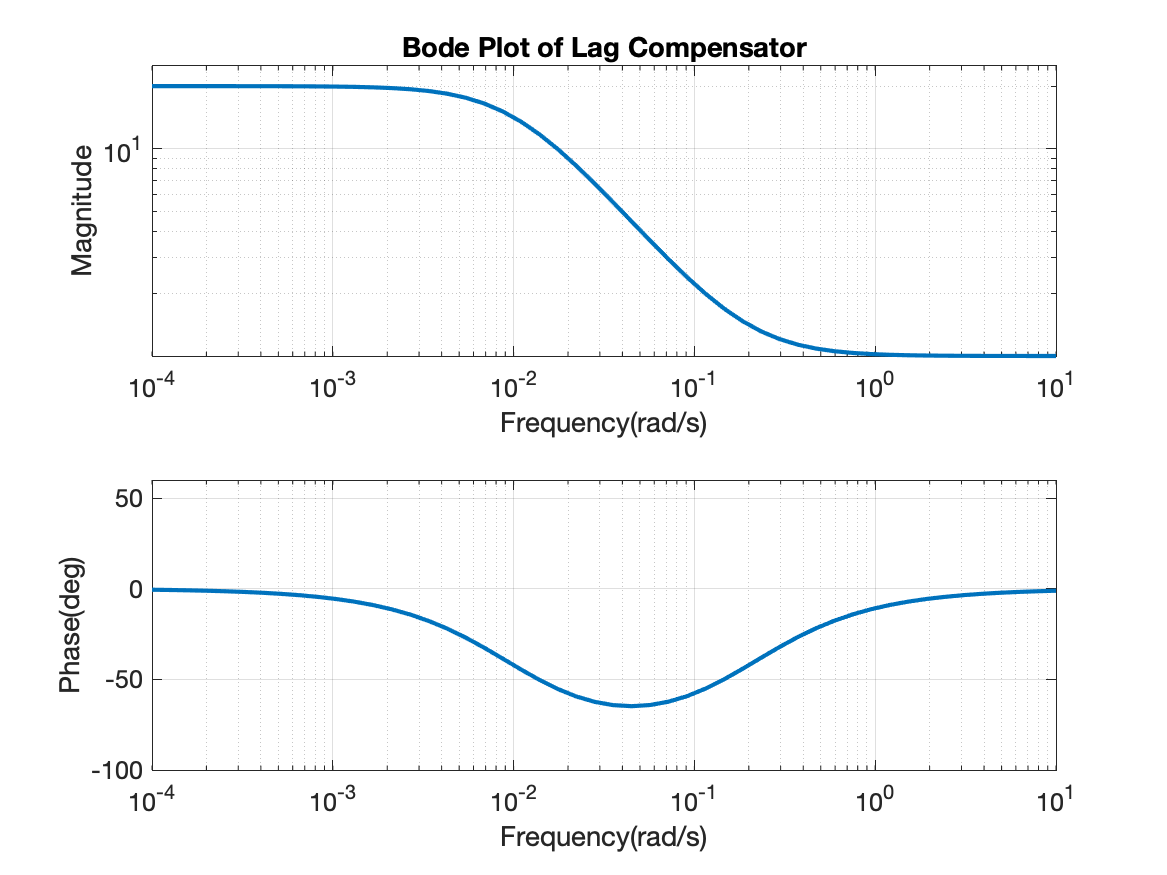
\includegraphics[width = 0.6\textwidth]{pic/1.png}
\end{figure}
\noindent Where the phase margin becomes about $\theta = 26.3^\circ$. So we need to more than $18.7^\circ$ to cover the requirement, that's why we need to introduce a lead compensator.
$$
D_{Lead} = \frac{T_Ds+1}{\alpha T_Ds +1}
$$
\noindent Where we choose $\phi_{max} = 33.7^\circ$, we have
$$
\alpha = \frac{1-\sin{\phi_{max}}}{1+\sin{\phi_{max}}} = 0.2865
$$
Adjusting $T_D = 1/(2.9\sqrt{\alpha}) = 0.6433$, we have the bode plot of Lead Compensator
\begin{figure}[H]
\centering
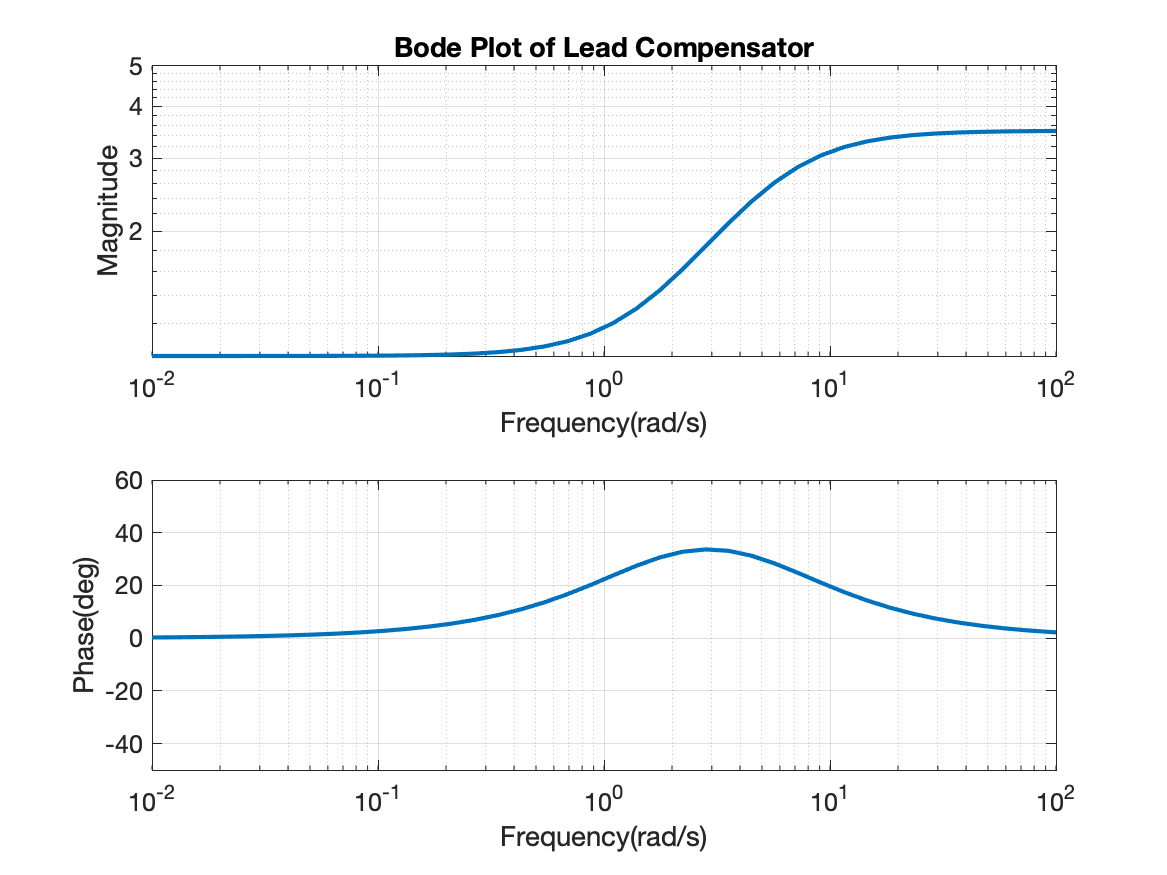
\includegraphics[width = 0.6\textwidth]{pic/2.png}
\end{figure}
\noindent Then we can see the gain margin is exactly $45^\circ$:
\begin{figure}[H]
\centering
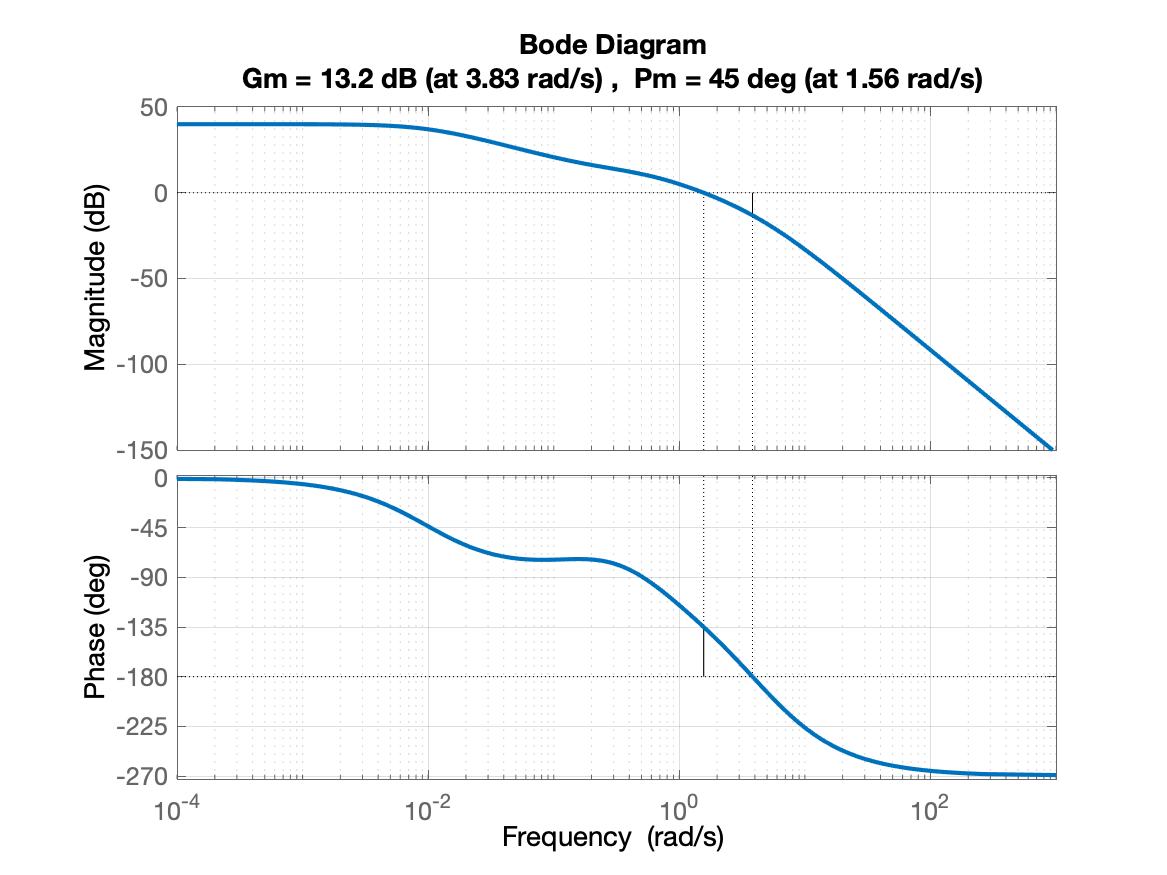
\includegraphics[width = 0.6\textwidth]{pic/5.png}
\end{figure}
\noindent Bode plot of the system with lead and lag, system with lag only, and system without controller, we can see the difference by adding different compensator.
\begin{figure}[H]
\centering
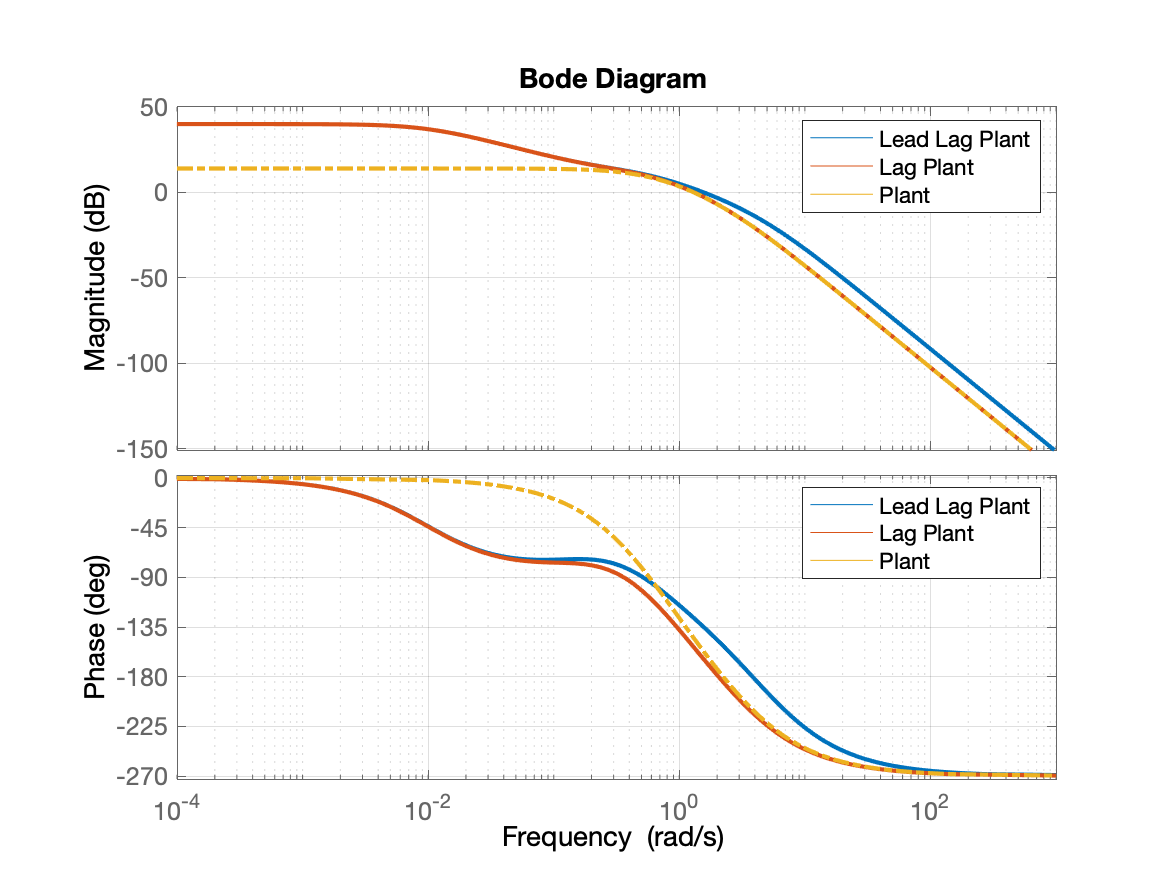
\includegraphics[width = 0.6\textwidth]{pic/3.png}
\end{figure}
Step response of the system with both lead and lag controller.
\begin{figure}[H]
\centering
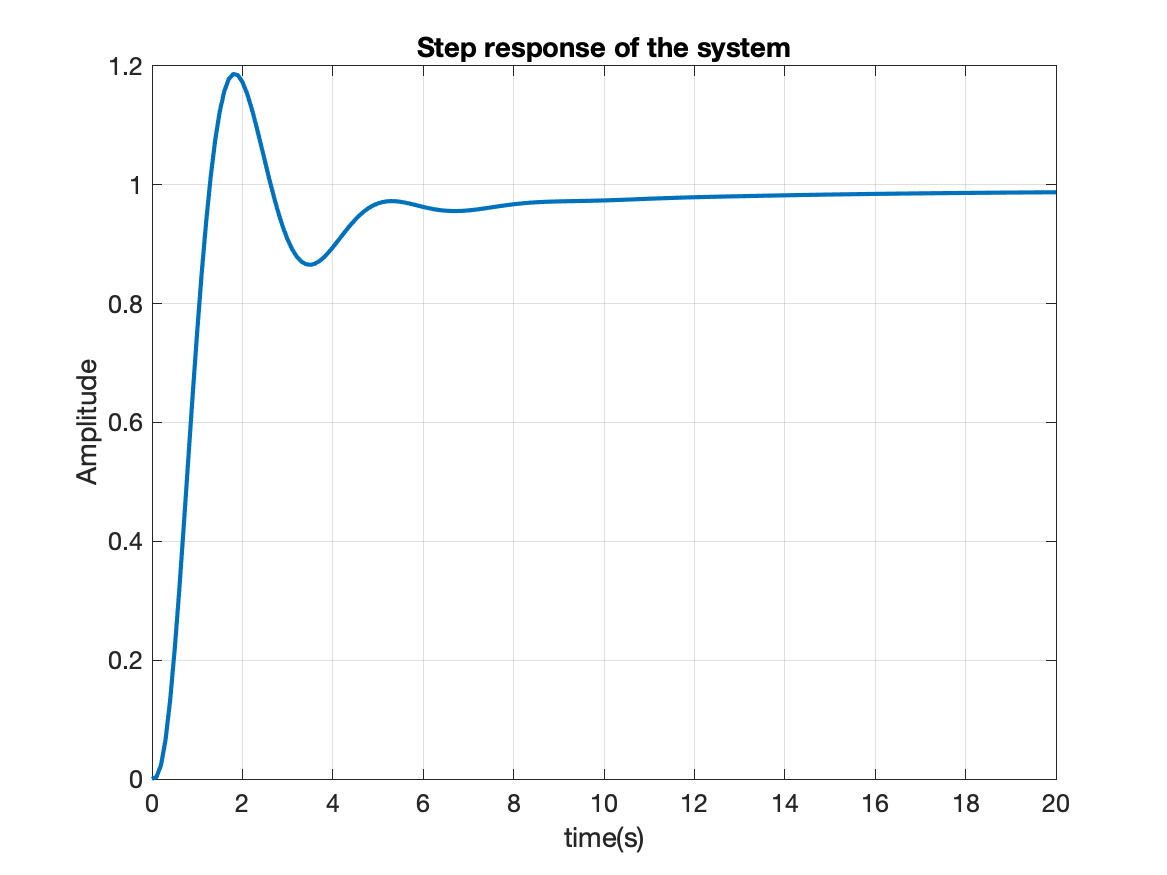
\includegraphics[width = 0.6\textwidth]{pic/4.png}
\end{figure}





\end{document}